\documentclass{article}

\usepackage{fancyhdr}
\usepackage{ragged2e}
\usepackage{graphicx}
\usepackage{caption}
\usepackage{geometry}
\usepackage{amsmath}
\usepackage{rotating}

\usepackage{listings}
\usepackage{color}

\definecolor{dkgreen}{rgb}{0,0.6,0}
\definecolor{gray}{rgb}{0.5,0.5,0.5}
\definecolor{mauve}{rgb}{0.58,0,0.82}

\lstset{frame=tb,
  language=Java,
  aboveskip=3mm,
  belowskip=3mm,
  showstringspaces=false,
  columns=flexible,
  basicstyle={\small\ttfamily},
  numbers=none,
  numberstyle=\tiny\color{gray},
  keywordstyle=\color{blue},
  commentstyle=\color{dkgreen},
  stringstyle=\color{mauve},
  breaklines=true,
  breakatwhitespace=true,
  tabsize=4
}

\setcounter{secnumdepth}{1}

\usepackage{chngcntr}
\counterwithin{figure}{section}

\renewcommand*{\thepage}{C\arabic{page}}

\pagestyle{fancy}
\lhead{ACME Robotics}
\chead{\#8367}
\rhead{\ifcontents Contents \else Week \thesection \fi}

\newif\ifcontents
\contentstrue

\makeatletter
\renewcommand{\@seccntformat}[1]{}
\makeatother

\begin{document}\contentsfalse

\subsection{Test vision software}
%! Develop vision software to detect the gold particle
Finding the gold particle at the beginning of the autonomous posed many challenges for the software team. Modifying a python vision script from the Relic Recovery season, Emma and Kelly were able to successfully detect the gold particle. However, the problems started when they realized that with the robot starting above the ground, the camera would have full view of the crater full of gold particles behind the line of particles they were trying to detect, as seen in
Figure \ref{fig:camera}.

After discussing possible solutions, including identifying the three particles first (both silver and gold), Emma decided to experiment with camera angles from approximately five inches above the field. Without having the field nor the mounting point on the robot, Emma tried her best to find the optimal position for the camera, although a final position will need to be determined once the robot is complete. 

Although there are different ways to solve this problem using programming, for simplicity's sake, Emma is hoping to troubleshoot more with the camera when the field arrives sometime in the next week. As they already have functional code, it would be beneficial to only have to position the camera correctly. 

\begin{figure}
    \centering
    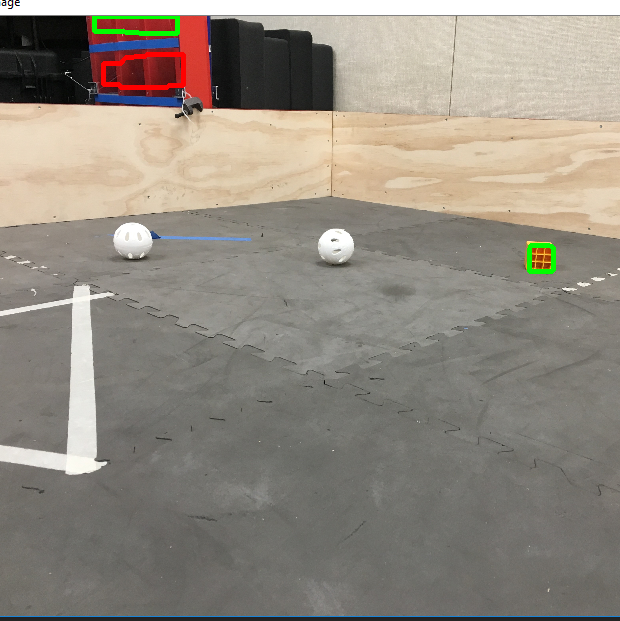
\includegraphics[width=.6\textwidth]{02_09-10/images/originalcameraposition.png}
    \caption{Original Position of the Camera}
    \label{fig:camera}
\end{figure}



\subsection{Experiment with new motor controller features} 
%! Play with new motor controller features to see what benefits they have.
New motor functionality added with v4.0 of the SDK and the new Rev Expansion Hub firmware has the ability to have a PIDF control loop on the Rev Hub itself. This means that rather than commanding some vague `power' to the motor, and then having to empirically determine the relationship between this power and the velocity of the motor, you can directly command a velocity, and the control loop on board the hub will match that velocity regardless of voltage droop. After upgrading the firmware in the hubs and testing this functionality with a lone motor, Kelly re-wrote the MecanumDrive class to take advantage of it. After deploying this to the Relic Recovery robot, Kelly found that the robot was much easier to control. Without any feed-back control on the robot controller side, the robot was very stable, and it was much easier to move the robot slowly, because the hub would now do the work of closing a loop around the velocity of the robot.
\end{document}